\begin{figure}[tbp]
\centering
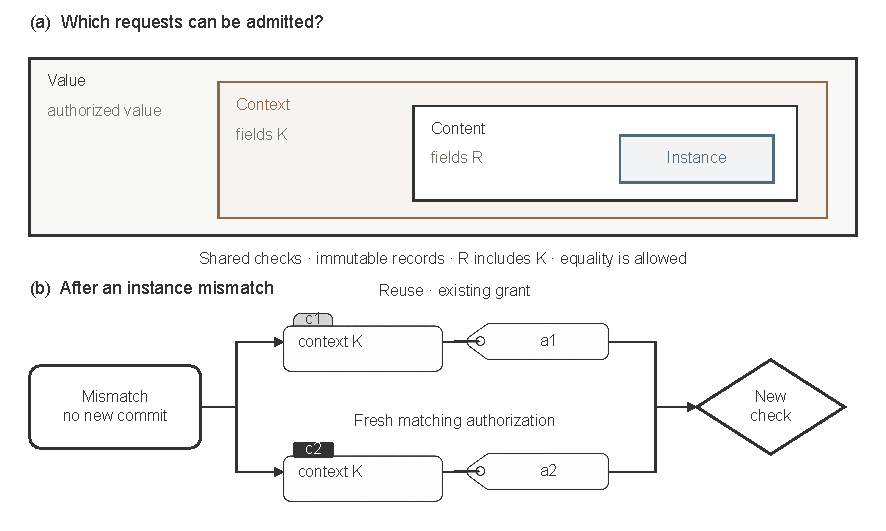
\includegraphics[width=\linewidth]{figures/fig3-design-space.pdf}
\caption{Binding and recovery are separate design choices. Under shared checks and content-immutable candidate records, if the compared content fields \(R\) include the retained context fields \(K\), the admissible request sets satisfy \(A_{\mathrm{instance}}\subseteq A_{\mathrm{content}}\subseteq A_{\mathrm{context}}\subseteq A_{\mathrm{value}}\). These inclusions need not be strict; context and content binding coincide when \(K=R\). Following an instance-mismatch rejection, the system may offer reuse of the reviewed candidate under the existing authorization or obtain matching authorization for another candidate. Reauthorization is a recovery branch, not another binding level. Each continuation must pass a new admission check; the schematic does not guarantee that an available route will be taken. Object glyphs were AI-generated; see the AI-assisted preparation declaration}
\label{fig:design}
\end{figure}
